%% 2/18/2016
%%%%%%%%%%%%%%%%%%%%%%%%%%%%%%%%%%%%%%%%%%%%%%%%%%%%%%%%%%%%%%%%%%%%%%%%%%%%
% AGUJournalSample.tex: this sample file is for articles formatted with LaTeX
%
% This sample file includes commands and instructions
% given in the order necessary to produce a final output that will
% satisfy AGU requirements.
%
% PLEASE DO NOT USE YOUR OWN MACROS
% DO NOT USE \newcommand, \renewcommand, or \def.
%
% FOR FIGURES, DO NOT USE \psfrag or \subfigure.
% DO NOT USE \psfrag or \subfigure commands.
%
%%%%%%%%%%%%%%%%%%%%%%%%%%%%%%%%%%%%%%%%%%%%%%%%%%%%%%%%%%%%%%%%%%%%%%%%%%%%
%
% All questions should be e-mailed to latex@agu.org.
%
%%%%%%%%%%%%%%%%%%%%%%%%%%%%%%%%%%%%%%%%%%%%%%%%%%%%%%%%%%%%%%%%%%%%%%%%%%%%
%
% Step 1: Set the \documentclass
%
% There are two options for article format:
%
% 1) PLEASE USE THE DRAFT OPTION TO SUBMIT YOUR PAPERS.
% The draft option produces double spaced output.
% 
% 2) numberline will give you line numbers.

% Tip:
%  To add line numbers to lines in equations:
%  \begin{linenomath*}
%  \begin{equation}
%  \end{equation}
%  \end{linenomath*}

%% To submit your paper:
\documentclass[linenumbers,draft]{agujournal}

% Now, type in the journal name: \journalname{<Journal Name>}
% ie,
\journalname{JGR-Atmospheres}

%% Choose from this list of Journals:
%
% JGR-Atmospheres
% JGR-Biogeosciences
% JGR-Earth Surface
% JGR-Oceans
% JGR-Planets
% JGR-Solid Earth
% JGR-Space Physics
% Global Biochemical Cycles
% Geophysical Research Letters
% Paleoceanography
% Radio Science
% Reviews of Geophysics
% Tectonics
% Space Weather
% Water Resource Research
% Geochemistry, Geophysics, Geosystems
% Journal of Advances in Modeling Earth Systems (JAMES)
% Earth's Future
% Earth and Space Science


%% ------------------------------------------------------------------------ %%
%
%  ENTER Title Page commands:
%
%% ------------------------------------------------------------------------ %%

% (A title should be specific, informative, and brief. Use
% abbreviations only if they are defined in the abstract. Titles that
% start with general terms then specific results are optimized in
% searches)

% Example: \title{This is a test title}

% (List authors by first name or initial followed by last name and
% separated by commas. Use \affil{} to number affiliations, and
% \thanks{} for author notes.  
% Additional author notes should be indicated with \thanks{} (for
% example, for current addresses). 

% Example: \authors{A. B. Author\affil{1}\thanks{Current address, Antartica}, B. C. Author\affil{2,3}, and D. E.
% Author\affil{3,4}\thanks{Also funded by Monsanto.}}

% (include name and email addresses of the corresponding author.  More
% than one corresponding author is allowed in this LaTeX file and for
% publication; but only one corresponding author is allowed in our
% editorial system.)  

%% Corresponding Author:
% Corresponding author mailing address and e-mail address:

% Example: \correspondingauthor{First and Last Name}{email@address.edu}

% Authors are individuals who have significantly contributed to the
% research and preparation of the article. Group authors are allowed, if
% each author in the group is separately identified in an appendix.)

% \affiliation{1}{First Affiliation}
% \affiliation{2}{Second Affiliation}
% \affiliation{3}{Third Affiliation}
% \affiliation{4}{Fourth Affiliation}

%% Keypoints, final entry on title page.
% Example: 
% \begin{keypoints}
% \item	List up to three key points (at least one is required)
% \item	Key Points summarize the main points and conclusions of the article
% \item	Each must be 100 characters or less with no special
% characters or punctuation 
% \end{keypoints}

%% \begin{abstract} begins second page 

%%%%%%%%%%%%%%%%%%%%%%%%%%%%%%%%%%%%%%%%%%%%%%%%%%%%%%%%%%%%%%%%%%%%%
% Track Changes:
% To add words, \added{<word added>}
% To delete words, \deleted{<word deleted>}
% To replace words, \replace{<word to be replaced>}{<replacement word>}
% To explain why change was made: \explain{<explanation>}

% At the end of the document, use \listofchanges, which will list the
% changes and the page and line number where the change was made.

% When final version, \listofchanges will not produce anything,
% \added{} word will be printed, \deleted{} will take away the word,
% \replaced{}{} will print only the 2nd argument.
% \explain will not print anything.

% Optional argument:
% You can also add additional information to be printed with the list
% of changes, to indicate the initials of the person changing the text,
% and the time and/or date of the change, or any other comment by using
% the optional [] argument:
% \added[AH, 3:30pm, Feb 18, 2016]{added term}
% will yield 
% [AH, 3:30pm, Feb 18, 2016] added term on page...
%%%%%%%%%%%%%%%%%%%%%%%%%%%%%%%%%%%%%%%%%%%%%%%%%%%%%%%%%%%%%%%%%%%%%

\begin{document}

%% ------------------------------------------------------------------------ %%
%
%  TITLE
%
%% ------------------------------------------------------------------------ %%


\title{Trends in the predictive performance of raw ensemble weather forecasts}


%% ------------------------------------------------------------------------ %%
%
%  AUTHORS AND AFFILIATIONS
%
%% ------------------------------------------------------------------------ %%

 \authors{A. B. Smith\affil{1}\thanks{Current address, McMurdo Station,
 Antartica},
 Eric Brown\affil{1,2}, Rick Williams\affil{3},
 John B. McDougall\affil{4}, and S. Visconti\affil{5}\thanks{Also
 funded by Monsanto.}}

\affiliation{1}{Department of Hydrology and Water Resources,
University of Arizona, Tucson, Arizona, USA.}
\affiliation{2}{Department of Geography, Ohio State University,
Columbus, Ohio, USA.}
\affiliation{3}{Department of Space Sciences, University of
Michigan, Ann Arbor, Michigan, USA.}
\affiliation{4}{Division of Hydrologic Sciences, Desert Research
Institute, Reno, Nevada, USA.}
\affiliation{5}{Dipartimento di Idraulica, Trasporti ed
Infrastrutture Civili, Politecnico di Torino, Turin, Italy.}


%% Corresponding Author
%(include name and email addresses of the corresponding author.  More
%than one corresponding author is allowed in this Word file and for
%publication; but only one corresponding author is allowed in our
%editorial system.)  

\correspondingauthor{A. B. Smith}{email@address.edu}

%  List up to three key points (at least one is required)
%  Key Points summarize the main points and conclusions of the article
%  Each must be 100 characters or less with no special characters or punctuation 

\begin{keypoints}
\item Evolution of raw ensemble forecast \replaced{skill}{skills}
\item Future benefits from statistical post-processing
\item Global distribution of forecast skill development
\end{keypoints}

%% ------------------------------------------------------------------------ %%
%
%  ABSTRACT
%
%% ------------------------------------------------------------------------ %%


\begin{abstract}
This study applies statistical post-processing to ensemble
forecasts of near-surface temperature, 24-hour 
%% below are examples of track changes:
\deleted[date/time, etc.]{precipitation},
\added{all} totals,
and near-surface wind speed from the global model of the European
Centre for Medium-Range Weather Forecasts (ECMWF). The main objective
is to evaluate the evolution of the difference in skill between the
raw ensemble and the post-processed forecasts. Reliability and
sharpness, and 
%% another example of track changes.
\replaced{hence}{therefore} skill,
 of the former is expected to improve over
time. Thus, the gain by post-processing is expected to decrease. Based
on ECMWF forecasts from January 2002 to March 2014 and corresponding
observations from globally distributed stations we generate
post-processed forecasts by ensemble model output statistics
%% another example of track changes.
\added{abbreviated as} (EMOS)
for each station and variable. Given the higher average skill of the
post-processed forecasts, we analyse the evolution of the difference
in skill between raw ensemble and EMOS. This skill gap remains almost
constant over time indicating that post-processing will keep adding
skill in the foreseeable future.
\end{abstract}

%% ------------------------------------------------------------------------ %%
%
%  TEXT
%
%% ------------------------------------------------------------------------ %%

%%% Suggested section heads:
% \section{Introduction}
% 
% The main text should start with an introduction. Except for short
% manuscripts (such as comments and replies), the text should be divided
% into sections, each with its own heading. 

% Headings should be sentence fragments and do not begin with a
% lowercase letter or number. Examples of good headings are:

% \section{Materials and Methods}
% Here is text on Materials and Methods.

% \subsection{A descriptive heading about methods}
% More about Methods.
% 
% \section{Data} (Or section title might be a descriptive heading about data)
% 
% \section{Results} (Or section title might be a descriptive heading about the
% results)
% 
% \section{Conclusions}


\section{Introduction}
\label{sec:intro}
Over the last two decades the paradigm in weather forecasting has
shifted from being deterministic to probabilistic \citep[see
e.g.][]{Palm00,Hami00}. Accordingly, numerical weather prediction
(NWP) models have been run increasingly as ensemble forecasting
systems. The goal of such ensemble forecasts is to approximate the
forecast probability distribution by a finite sample of scenarios
\citet{Leit74}\footnote{See \citet{Leit74} for a more in-depth
description of these issues and their complex implications.}
Global ensemble forecast systems, like the European
Centre for Medium-Range Weather Forecasts (ECMWF) ensemble, are prone
to probabilistic biases, and are therefore not reliable. They
particularly tend to be underdispersive for surface weather parameters
\citet{Boug10, Park08}. In order to correct for forecast
underdispersion and bias in NWP ensembles different
statistical
post-processing methods have been developed, of which ensemble model
output statistics (EMOS) \citep{Gneit05} is among the most widely
applied. EMOS yields a parametric forecast distribution by linking its
parameters to ensemble statistics. Due to its simplicity and low
computational cost, we focus on EMOS for this study.



The ECMWF ensemble is under continuous development, and hence its
forecast skill improves over time \citep{Buiz98,Buiz07,Rich13,Haid14}.
Parts of these improvements may be due to a reduction of probabilistic
biases. From this we deduce the following hypothesis: As the raw
forecasts continuously improve, it is hypothesized that the gap in
skill between raw ensemble and post-processed forecasts narrows,
because systematic errors typically captured by post-processing are
reduced 
by those improvements. 
%%
%% Use \explain{} before change, so that it ends up on the right line.
\explain[Jon, 2/16/16]{Redundant sentence, better without it} 
\deleted{In other words, probabilistic biases,
which can be reduced by statistical post-processing methods, decrease
over time.}
Assuming that the raw ensemble forecasts continue to
improve in the future, the gap in skill may eventually be closed when
the raw ensemble forecasts become reliable and unbiased.  In this work
we analyse the evolution of the global performance of the operational
ECMWF raw ensemble and the corresponding post-processed EMOS forecasts
for 2 metre temperature (T2M), 24-hour precipitation (PPT24), and 10-m
wind speed (V10). We verify the forecasts against globally distributed
surface synoptic observations (SYNOP) data over a period of about 10
years. We firstly evaluate the monthly average skill in terms of CRPS
for both the raw and the EMOS forecasts. In order to assess the extent
to which the results depend on the choice of the post-processing
method, Bayesian model averaging (BMA), \citet{Raft05,Fra10} is
additionally applied to the T2M raw ensemble forecasts. We will use
the negatively oriented (i.e. the lower the value the higher the
skill) continuous ranked probability score (CRPS) \citep{Math76} as a
measure of skill. As the CRPS assesses both reliability and sharpness
and is a proper score \citep{Gneit07b}, we rely on it for model fitting
and verification throughout this study. Note that skill and
reliability are linked in that given constant sharpness an improvement
in reliability leads to an improvement in skill and vice versa. We
finally analyse the evolution of the gap in CRPS between raw ensemble
and post-processed forecasts.

After presenting the dataset in section~\ref{sec:intro} we summarize
the methods for post-processing and for the assessment of the global
skill evolution in section~\ref{sec:meth}. In section~\ref{sec:res}
the results are shown.  This is followed by a discussion in
section~\ref{sec:disc} along with some concluding
remarks. These
analyses have been performed using the statistical software \texttt{R}
\citep{R2013}.


%% Enter Figures and Tables near as possible to where they are first mentioned:
%
% DO NOT USE \psfrag or \subfigure commands.
%
% Figure captions go below the figure.
% Table titles go above tables;  other caption information
%  should be placed in last line of the table, using
% \multicolumn2l{$^a$ This is a table note.}
%
%----------------
% EXAMPLE FIGURE
%
% \begin{figure}
% \end{figure}

\begin{figure}[ht!]
% \centering
% when using pdflatex, use pdf file:
% 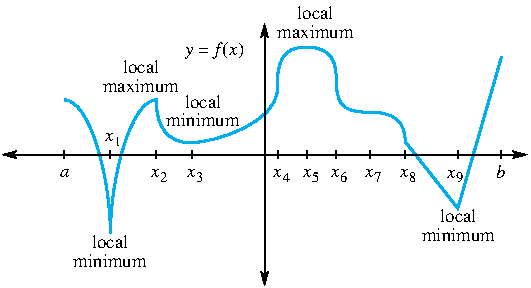
\includegraphics[width=20pc]{figsamp.pdf}
%
% when using dvips, use .eps file:
% 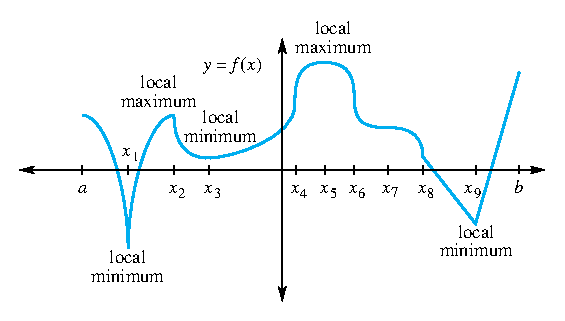
\includegraphics[width=20pc]{figsamp.eps}
%
% If you don't specify the file extension, 
% \includegraphics will insert the right file:
\centerline{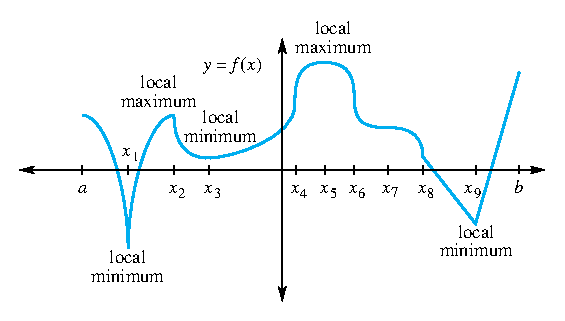
\includegraphics[height=1.5in]{figsamp}}
\caption{Short caption}
\label{figone}
\end{figure}

\begin{figure}[ht!]
\centerline{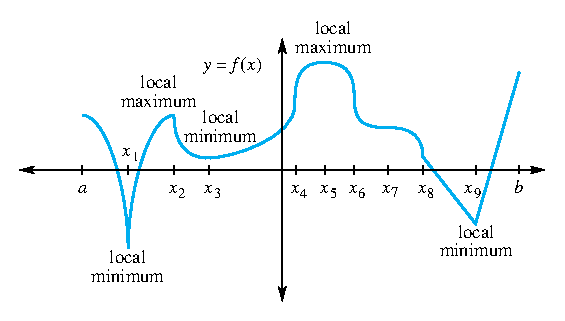
\includegraphics[angle=45,height=2in]{figsamp}}
\caption{The figure caption should begin with an overall descriptive
statement of the figure followed by additional text. They should be
immediately after each figure.  Figure parts are indicated with
lower-case letters ({\bf a, b, c}\ldots).  For initial submission, please place
both the figures and captions in the text near where they are cited.}
\label{fig:mean_and_slope}
\end{figure}


\begin{table}
\caption{Start this caption with a short description of your
table.
Large tables
especially presenting rich data should be presented as separate excel
or .cvs files, not as part of the main text.}
== Table Here ==
\end{table}

%
% ---------------
% EXAMPLE TABLE
%
\begin{table}
\caption{Time of the Transition Between Phase 1 and Phase 2$^{a}$}
\centering
\begin{tabular}{l c}
\hline
 Run  & Time (min)  \\
\hline
  $l1$  & 260   \\
  $l2$  & 300   \\
  $l3$  & 340   \\
  $h1$  & 270   \\
  $h2$  & 250   \\
  $h3$  & 380   \\
  $r1$  & 370   \\
  $r2$  & 390   \\
\hline
\multicolumn{2}{l}{$^{a}$Table note text here.}
\end{tabular}
\end{table}


% See below for how to make sideways figures or tables.

% AGU prefers the use of {sidewaystable} over {landscapetable} as it causes fewer problems.
%
 \begin{sidewaysfigure}
 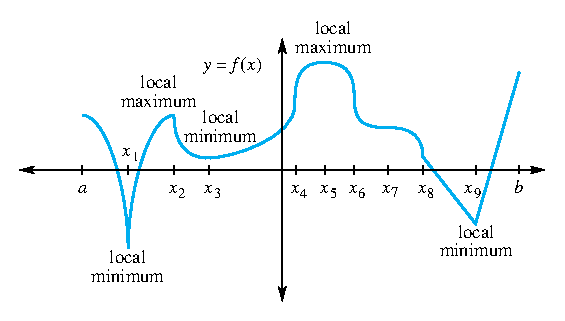
\includegraphics[width=20pc]{figsamp}
 \caption{Caption here}
 \label{newfig}
 \end{sidewaysfigure}
%
 \begin{sidewaystable}
 \caption{Caption here}
\label{tab:signif_gap_clos}
 \begin{tabular}{ccc}
one&two&three\\
four&five&six
 \end{tabular}
 \end{sidewaystable}

\clearpage

\section{Methods}
\label{sec:meth}

\subsection{Post-processing Using EMOS}
Post-processing using EMOS converts a raw ensemble of discrete
forecasts into a probability distribution. Let $y$ be the variable to
be forecast (here: T2M, PPT24 or V10) and let ${f}=(f_{1}, f_{2},
\dots, f_{K})^{T}$ be the vector of the $K$ member raw ensemble
forecasts (here: HRES, ENS, and CTRL). Then the EMOS
\added{predictive}
density can be written as:
\begin{linenomath*}
\begin{equation}
y|{f} \sim g(m, \sigma),
\end{equation}
\end{linenomath*}
where $g(\cdot)$ is a parametric density function with location and
scale parameters $m$ and $\sigma$, respectively, which depend on the
raw ensemble.

\subsubsection{Temperature}
For T2M forecasts $g(\cdot)$ is a normal density distribution with
mean $m$ and variance $\sigma^{2}$. Here, we use a variant of the
original EMOS approach similar to the one proposed by
\citet{ScheueBue13} where the departures of observed temperatures from
their climatological means are related to those of the forecasts.
Specifically, let $T=\{t_{1},\ldots,t_{n}\}$ be a training period of
$n$ days preceding the forecast initialization and denote by $f_{tk}$
the forecast of the k-th ensemble member and by $y_{t}$ the
observation on day $t\in T$. As a first step, we fit a regression
model
%%% \begin{linenomath*} ...\end{linenomath*} puts a line number in equation:
\begin{linenomath*}
\begin{equation}
y_{t_{j}} = c_{0} + c_{1}\sin\left(\frac{2\pi j}{365}\right) +
c_{2}\cos\left(\frac{2\pi j}{365}\right) + \varepsilon_{t_{j}}, \quad
j=1,\ldots,n
\end{equation}
\end{linenomath*}
which captures the seasonal variation of T2M. The residual terms
$\varepsilon_{t_{j}}$ are likely correlated over time, but for
simplicity an ordinary least squares fit is performed. We denote by
$\tilde{y}_{t}$ the fitted value of this periodic regression model on
day $t$ and interpret it as the climatological mean temperature on
this day. This model can easily be extrapolated to future days
$t_{d+1}, t_{d+2}, \ldots$ The above regression includes both a sine
and a cosine term which is equivalent to a cosine model with variable
phase and amplitude. Since $j=1,\ldots,n$ is just a numbering of the
days in $T$, different training periods have different phase
parameters and hence $c_{1}$ and $c_{2}$ evolve over the calendar
year. We fit the same type of model also to the ensemble mean,
control, and high resolution run and obtain climatological means
$\tilde{f}_{\overline{\mathrm{ENS}},t}, \tilde{f}_{\mathrm{CTRL},t}$,
and $\tilde{f}_{\mathrm{HRES},t}$. The mean of the forecast
distribution is then:
\begin{linenomath*}
\begin{equation}
m = \tilde{y} + a_{1}(f_{\mathrm{HRES}} - \tilde{f}_{\mathrm{HRES}}) +
a_{2}(f_{\mathrm{CTRL}} - \tilde{f}_{\mathrm{CTRL}}) +
a_{3}(f_{\overline{\mathrm{ENS}}} -
\tilde{f}_{\overline{\mathrm{ENS}}}).
\end{equation}
\end{linenomath*}
The variance of the forecast distribution is linked to the raw
ensemble by: 
\begin{linenomath*}
\begin{equation}
\sigma^{2} = b_{0} + b_{1}s^{2},
\end{equation}
\end{linenomath*}
where $s^{2} = \frac{1}{K}\sum_{k=1}^{K}(f_{k} -
\frac{1}{K}\sum_{k=1}^{K}f_{k})^{2}$. The parameters
${\theta}_{T2M}=(a_{1}, a_{2}, a_{3}, b_{0}, b_{1})^{T}$ are
constrained to be non-negative, and hence $a_{k}/\sum_{k=1}^{K} a_{k}$
can be understood as the weight of model $k$.

\subsubsection{Precipitation}
For PPT24 we use the EMOS approach proposed by \citet{Scheu14}, where
$g(\cdot)$ is a left-censored (at zero) generalized extreme value
(GEV) distribution. While the shape parameter $\xi$ of the GEV is kept
constant ($\xi=0.2$), the location and the scale parameters $m$ and
$\sigma$ are linked to the raw ensemble via:
\begin{linenomath*}
\begin{eqnarray}
m &=& a_{0} + a_{1} f_{\mathrm{HRES}} + a_{2} f_{\mathrm{CTRL}} +
a_{3} f_{\overline{\mathrm{ENS}}} + a_{4} \pi_{0},\nonumber\\
\sigma &=& b_{0} + b_{1} \mathrm{MD}_{f},
\end{eqnarray}
\end{linenomath*}
where $\pi_{0}$ is the fraction of ensemble members predicting zero
precipitation and $\mathrm{MD}_{f}:= K^{-2}$\break
$\sum_{k, k' = 1}^{K} |
f_{k} - f_{k'} |$ is the ensemble mean difference. Again, the
parameters are denoted by $\theta_{PPT24}=(a_{0}, \dots, a_{4}, b_{0},
b_{1})^{T}$. The parameters $a_{1}, a_{2}, a_{3}, b_{0}, b_{1}$ are
constrained to be non-negative, and hence the normalized parameters
$a_{1}$ to $a_{3}$ can be understood as weights.

\subsection{Global CRPS Analysis}
 \label{sec:meth_glob_crps}

As stated in the introduction, the main objective of this study is to
analyse whether the gap in CRPS between the raw ensemble and the
post-processed forecast narrows over time. This is assessed
station-wise using both a parametric and a non-parametric approach.
For the former, we fit the following regression model to the monthly
time series of CRPS differences ($\Delta \mathrm{CRPS}_{t} =
\mathrm{CRPS}_{\mathrm{raw},t} - \mathrm{CRPS}_{\mathrm{EMOS}, t}$):
\begin{linenomath*}
\begin{equation}
\Delta \mathrm{CRPS}_{t} = \beta_{0} + \beta_{1} t + \beta_{2} \sin\left(\frac{2\pi t}{12}\right) + \beta_{3} \cos\left(\frac{2\pi t}{12} \right) + \epsilon, \phantom{bla} \epsilon \sim \mathcal{N}(0, \sigma^{2}) \label{eq:linseas}
\end{equation}
\end{linenomath*}
where $\Delta \mathrm{CRPS}_{t}$ is the predictand, $t$ is now the
time in months, and $\sigma^{2}$ denotes the error variance. For the
latter, we use Kendall's $\tau$ correlation coefficient and the
associated test statistics \citep{Mann45} as implemented in the
\texttt{R} package \texttt{Kendall} \citep{Kendall}. In order to
correct for seasonal effects, we calculate the $\tau$ statistics using
the residuals of the following model:
\begin{linenomath*}
\begin{equation}
\Delta \mathrm{CRPS}_{t} = \gamma_{0} + \gamma_{1} \sin\left(\frac{2\pi t}{12}\right) + \gamma_{2} \cos\left(\frac{2\pi t}{12} \right) + \epsilon, \phantom{bla} \epsilon \sim \mathcal{N}(0, \sigma^{2})
\label{eq:tauseas}
\end{equation}
\end{linenomath*}
Note that negative $\tau$ values indicate a negative trend and
positive values a positive one. Figure~\ref{figone} a) and b)
show the regression lines estimated by model (\ref{eq:linseas}) for
monthly averages of $\Delta \mathrm{CRPS}$ and the corresponding
Kendall's $\tau$ test statistics for an example with decreasing and
increasing gap.


\section{Results}
\label{sec:res}

\subsection{Are There Any Significant Temporal Trends?}


The above results indicate a tendency of a decrease in $\Delta$CRPS
over time at least for T2M and PPT24. In the following we check the
percentages of stations with decreasing, an absence of, or increasing
trend in $\Delta$CRPS over time at a significance level of 0.05. In
order to be more confident about the results this analysis is
performed using both the parametric regression model and the
non-parametric Kendall's $\tau$ correlation coefficient test. As
already mentioned both approaches correct for seasonal effects.
Furthermore, in case of T2M the same analysis has been performed
additionally using BMA instead of EMOS in order to relax the
dependence on one particular post-processing method. As shown in
Table~\ref{tab:signif_gap_clos} the stations with no significant trend
outnumber the stations with either negative or positive trend for all
three variables and lead times considered. Note that the percentage of
stations without any significant trend increases with increasing lead
time. In line with the results shown in
Figure~\ref{fig:mean_and_slope}, significantly negative trends are
more common than positive ones for T2M and PPT24. The difference
between the number of stations with negative and those with positive
trend reduces with increasing lead time, but is still greater than
zero for a 10 day forecast. Note that the high number of
non-significant stations in case of PPT24 is likely to be due to the
high variability of precipitation amounts, and hence variability of
CRPS values, which leads to a large residual standard error in case of
the parametric regression model and to a lot of pairs (a pair denotes
here a value of $\Delta$CRPS and its associated time stamp) opposite
to the estimated direction in case of the $\tau$ test statistics. In
case of V10 the stations with a negative trend and those with a
positive trend are almost equally frequent regardless of the lead
time. Figures of the global distributions of stations with no,
significantly negative, and significantly positive trend in
$\Delta$CRPS are available as supplemental material to this paper.


\section{Discussion and Conclusions}
\label{sec:disc}

According to the above analyses the gap in CRPS between the raw
ensemble and the EMOS forecasts remains almost constant over time. For
T2M and PPT24 $\Delta$CRPS shows a slightly decreasing tendency. The
higher the lead time the less accentuated is this tendency. For V10
such a tendency cannot be detected. The parametric regression model
and the non-parametric $\tau$ test yield similar results. Hence, a
linear model that is overlaid by seasonal fluctuations seems to be
reasonable. Note that the skill of the raw ensemble and the EMOS
forecasts may sometimes be negatively affected by upgrades to the
atmospheric model. Model upgrades may deteriorate raw ensemble skill
at some individual stations. For instance, a resolution increase may
introduce new issues with statistical downscaling of the forecasts to
some specific observation sites. But more importantly, the skill of
the post-pro\-cessed forecasts can be lowered dramatically if a model
update happens between the training and the verification period. These
issues may result in positive trends in $\Delta$CRPS. Ideally,
post-processing would be based on a cascade of reforecasts. That is,
for each atmospheric model version, training of the post-processing
model would be done using a corresponding time series of reforecasts
made with that same model version. Furthermore, the observations may
be affected by measurement errors. If these errors change over time,
they may also influence the estimates of the trends in $\Delta$CRPS.
As the problems introduced by statistical downscaling may be mitigated
by verifying against model analysis, a similar study that replaces
observations by model analysis, as proposed by \citet{Ghel00} and
\citet{Papp09}, may give further insights.

From the above we conclude that the probabilistic skill of both the
raw ensembles and the EMOS forecasts improves over time. The fact that
the gap in skill has remained almost \textbf{constant}, especially for
V10, suggests that improvements to the atmospheric model have an
effect quite different from what calibration by statistical
post-processing is doing. That is, they are increasing potential
skill. Thus this study indicates that (a) further model development is
important even if one is just interested in point forecasts, and (b)
statistical post-processing is important because it will keep adding
skill in the foreseeable future.

%% ------------------------------------------------------------------------ %%
\section*{Citations}

% Please use ONLY \citet and \citep for reference citations.
% DO NOT use other cite commands (e.g., \cite, \citeyear, \nocite, \citealp, etc.).

\subsection*{Cites made with \tt\string\citet\string{\string}}
...as shown by \citet{Boug10}, \citet{Buiz07}, \citet{Fra10},
\citet{Ghel00}, and \citet{Leit74}. 

\subsection*{Cites made with \tt\string\citep\string{\string}}
...as shown by \citep{Boug10}, \citep{Buiz07}, \citep{Fra10},
\citep{Ghel00, Leit74}. 

...has been shown \citep [e.g.,][]{Boug10,Buiz07,Fra10}.




%%% End of body of article

%%%%%%%%%%%%%%%%%%%%%%%%%%%%%%%%
%% Optional Appendix goes here
%
% \appendix resets counters and redefines section heads
% but doesn't print anything.
% After typing \appendix
%
%\section{Here Is Appendix Title}
% will show
% A: Here Is Appendix Title
%
\appendix
\section{Here is a sample appendix}
This is an Appendix section.

\subsection{subsection}
This is an Appendix subsection.

\subsubsection{subsubsection}
This is an Appendix subsubsection.
\begin{linenomath*}
\begin{equation}asdf\end{equation}
\end{linenomath*}

%%%%%%%%%%%%%%%%%%%%%%%%%%%%%%%%%%%%%%%%%%%%%%%%%%%%%%%%%%%%%%%%
%
% Optional Glossary, Notation or Acronym section goes here:
%
%%%%%%%%%%%%%%
% Glossary is only allowed in Reviews of Geophysics
\begin{glossary}
\term{Term}
 Term Definition here
\term{Term}
 Term Definition here
\term{Term}
 Term Definition here
\end{glossary}

%
%%%%%%%%%%%%%%
% Acronyms
 \begin{acronyms}
 \acro{Acronym}
 Definition here
 \acro{EMOS}
 Ensemble model output statistics 
 \acro{ECMWF}
 Centre for Medium-Range Weather Forecasts
 \end{acronyms}

%
%%%%%%%%%%%%%%
% Notation 
 \begin{notation}
 \notation{$a+b$} Notation Definition here
 \notation{$e=mc^2$} 
 Equation in German-born physicist Albert Einstein's theory of special
relativity that showed that the increased relativistic mass ($m$) of a
body comes from the energy of motion of the body—that is, its kinetic
energy ($E$)—divided by the speed of light squared ($c^2$).
 \end{notation}




%%%%%%%%%%%%%%%%%%%%%%%%%%%%%%%%%%%%%%%%%%%%%%%%%%%%%%%%%%%%%%%%
%
%  ACKNOWLEDGMENTS

\acknowledgments
The forecast data used in this study can be made available subject to
a handling charge. SYNOP observations are not available through ECMWF.
We are grateful to F. Rabier, D. S. Richardson, D. Lavers, and other
colleagues at ECMWF for helpful discussions and inputs. We thank David
M\"{o}ller of the University of Heidelberg for his contribution.
Furthermore, we like to thank T. Gneiting of the Heidelberg Institute
for Theoretical Studies and of the Institute for Stochastics at
Karlsruhe Institute of Technology for valuable comments, and the
colleagues at the Heidelberg Institute for Theoretical Studies.
Additionally, we are grateful to two anonymous reviewers for their
helpful comments. We are indebted to the ECMWF for granting access to
their products.

The Editor thanks Pierre Pinson and an anonymous reviewer for their assistance in evaluating this paper.




%%  REFERENCE LIST AND TEXT CITATIONS
%
% Either type in your references using
%
% \begin{thebibliography}{}
% \bibitem{}
% Text
% \end{thebibliography}
%
% Or, to use BibTeX:
%
% Follow these steps
%
% 1. Type in \bibliography{<name of your .bib file>} 
%    Run LaTeX on your LaTeX file.
%
% 2. Run BiBTeX on your LaTeX file.
%
% 3. Open the new .bbl file containing the reference list and
%   copy all the contents into your LaTeX file here.
%
% 4. Run LaTeX on your new file which will produce the citations.
%
% AGU does not want a .bib or a .bbl file. Please copy in the contents of your .bbl file here.


\begin{thebibliography}{}

\bibitem[{\textit{Bell and Munoz}}(2008)]{Boug10} Bell, A.~H., and
Munoz, D.~P.  (2008). Activity in the superior colliculus reflects
dynamic interactions between voluntary and involuntary influences on
orienting behaviour. \textit{Eur. J. Neurosci.} 28, 1654--1660.

\bibitem[{\textit{Corbetta et~al.}}(1991)]{Buiz07} Corbetta, M.,
Miezin, F.~M., Dobmeyer, S., Shulman, G.~L., and Petersen, S.~E.
(1991). Selective and divided attention during visual discriminations
of shape, color, and speed: functional anatomy by positron emission
tomography. \textit{J.~Neurosci.} 11, 2383--2402.

\bibitem[{\textit{Borra et~al.}}(2014)]{Buiz98} Borra, E., Gerbella,
M., Rozzi, S., Tonelli, S., and Luppino, G.  (2014). Projections to
the superior colliculus from inferior parietal, ventral premotor, and
ventrolateral prefrontal areas involved in controlling goal-directed
hand actions in the macaque. \textit{Cereb. Cortex} 24, 1054--1065.

\bibitem[{\textit{Dorris et~al.}}(1997)]{Fra10}
 Dorris, M.~C.,
Par\'{e}, M., and Munoz, D.~P.  (1997). Neuronal activity in monkey
superior colliculus related to the initiation of saccadic eye
movements. \textit{J.~Neurosci.} 17, 8566--8579.

\bibitem[{\textit{Elsabbagh et~al.}}(2009)]{Ghel00} 
Elsabbagh, M.,
Volein, A., Holmboe, K., Tucker, L., Csibra, G., Baron-Cohen, S.,
et~al.  (2009). Visual orienting in the early broader autism
phenotype: disengagement. \textit{J.~Child Psychol. Psychiatry} 50,
637--642.

\bibitem[{\textit{Fortin et~al.}}(1999)]{Gneit05} Fortin, S., Chabli,
A., Dumont, I., Shumikhina, S., Itaya, S.~K., and Molotchnikoff, S.
(1999). Maturation of visual receptive field properties in the rat
superior colliculus. \textit{bibain Res. Dev. Brain Res.} 1112,
55--64.

\bibitem[{\textit{Felsen and Mainen}}(2008)]{Gneit07b} Felsen, G., and
Mainen, Z.~F.  (2008). Neural substrates of sensory-guided locomotor
decisions in the rat superior colliculus. \textit{Neuron} 60,
137--148.

\bibitem[{\textit{Gattass and Desimone}}(1996)]{Haid14} Gattass, R.,
and Desimone, R.  (1996). Responses of cells in the superior
colliculus during performance of a spatial attention task in the
macaque. \textit{Rev. Bras. Biol.} 56, 257--279.

\bibitem[{\textit{Goldberg and Wurtz}}(1972)]{Hami00} Goldberg, M.~E.,
and Wurtz, R.~H.  (1972). Activity of superior colliculus in behaving
monkey. II. Effect of attention on neuronal responses.
\textit{J.~Neurophysiol.} 35, \hbox{560--574}.

\bibitem[{\textit{Krauzlis}}(2003)]{Kendall} Krauzlis, R.~J.  (2003).
Neuronal activity in the rostral superior colliculus related to the
initiation of pursuit and saccadic eye movements.
\textit{J.~Neurosci.} 23, 4333--4344.

\bibitem[{\textit{Heesy}}(2009)]{Leit74} 
Heesy, C.~P.  (2009). Seeing
in stereo: the ecology and evolution of primate binocular vision and
stereopsis. \textit{Evol. Anthropol.} 18, 21--35.

\bibitem[{\textit{Hilbig et~al.}}(2000)]{Mann45} Hilbig, H., Bidmon,
H.~J., Ettrich, P., and M\"{u}ller, A.  (2000). Projection neurons in
the superficial layers of the superior colliculus in the rat: a
topographic and quantitative morphometric analysis.
\textit{Neuroscience} 96, 109--119.

\bibitem[{\textit{Ignashchenkova et~al.}}(2004)]{Math76}
Ignashchenkova, A., Dicke, P.~W., Haarmeier, T., and Their, P.
(2004). Neuron-specific contribution of the superior colliculus to
overt and covert shifts of attention. \textit{Nat. Neurosci.} 7,
56--64.

\bibitem[{\textit{Krauzlis et~al.}}(2013)]{Palm00} Krauzlis, R.~J.,
Lovejoy, L.~P., and Z\'{e}non, A.  (2013). Superior colliculus and
visual spatial attention. \textit{Annu. Rev. Neurosci.} 36, 165--182.

\bibitem[{\textit{Kustov and Robinson}}(1996)]{Papp09} Kustov, A.~A.,
and Robinson, D.~L.  (1996). Shared neural control of attentional
shifts and eye movements. \textit{Nature} 384, 74--77.

\bibitem[{\textit{Landry and Bryson}}(2004)]{Park08} Landry, R., and
Bryson, S.~E.  (2004). Impaired disengagement of attention in young
children with autism. \textit{J.~Child Psychol. Psychiatry} 45,
1115--1122.

\bibitem[{\textit{Kobayashi et~al.}}(2003)]{R2013} Kobayashi, T.,
Tran, A.~H., Nishijo, H., Ono, T., and Matsumoto, G.  (2003).
Contribution of hippocampal place cell activity to learning and
formation of goal-directed navigation in rats. \textit{Neuroscience}
117, 1025--1035.

\bibitem[{\textit{McHaffie et~al.}}(2005)]{Raft05} McHaffie, J.~G.,
Stanford, T.~R., Stein, B.~E., Coizet, V., and Redgrave, P.  (2005).
Subcortical loops through the basal ganglia. \textit{Trends Neurosci.}
28, 401--407.

\bibitem[{\textit{McPeek and Keller}}(2004)]{Rich13} McPeek, R.~M.,
and Keller, E.~L.  (2004). Deficits in saccade target selection after
inactivation of superior colliculus. \textit{Nat. Neurosci.} 7,
757--763.

\bibitem[{\textit{M\"{u}ller et~al.}}(2005)]{Scheu14} M\"{u}ller,
J.~R., Philiastides, M.~G., and Newsome, W.~T.  (2005).
Microstimulation of the superior colliculus focuses attention without
moving the eyes. \textit{Proc. Natl. Acad. Sci. U.S.A.} 102, 524--529.

\bibitem[{\textit{Munoz and Istvan}}(1998)]{ScheueBue13} Munoz, D.~P.,
and Istvan, P.~J.  (1998). Lateral inhibitory interactions in
the intermediate layers of the monkey superior colliculus.
\textit{J.~Neurophysiol.} 79, 1193--1209.

\end{thebibliography}

%%%%%%%%%%%%%%%%%%%%%%%%%%%%%%%%%%%%%%%%%
% Track Changes:
% To add words, \added{<word added>}
% To delete words, \deleted{<word deleted>}
% To replace words, \replace{<word to be replaced>}{<replacement word>}

% At the end of the document, use \listofchanges, which will list the
% changes and the page and line number where the change was made.

% When final version, \listofchanges will not produce anything,
% \added{} word will be printed, \deleted{} will take away the word,
% \replaced{}{} will print only the 2nd argument.

%%%
\listofchanges
%%%

\end{document}

%%%%%%%%%%%%%%%%%%%%%%%%%%%%%%%%%%%%%
%% Supporting Information
%% (Optional) See AGUSuppInfoSamp.tex/pdf for requirements 
%% for Supporting Information.
%%%%%%%%%%%%%%%%%%%%%%%%%%%%%%%%%%%%%


%%%%%%%%%%%%%%%%%%%%%%%%%%%%%%%%%%%%%%%%%%%%%%%%%%%%%%%%%%%%%%%

More Information and Advice:

%% ------------------------------------------------------------------------ %%
%
%  SECTION HEADS
%
%% ------------------------------------------------------------------------ %%

% Capitalize the first letter of each word (except for
% prepositions, conjunctions, and articles that are
% three or fewer letters).

% AGU follows standard outline style; therefore, there cannot be a section 1 without
% a section 2, or a section 2.3.1 without a section 2.3.2.
% Please make sure your section numbers are balanced.
% ---------------
% Level 1 head
%
% Use the \section{} command to identify level 1 heads;
% type the appropriate head wording between the curly
% brackets, as shown below.
%
%An example:
%\section{Level 1 Head: Introduction}
%
% ---------------
% Level 2 head
%
% Use the \subsection{} command to identify level 2 heads.
%An example:
%\subsection{Level 2 Head}
%
% ---------------
% Level 3 head
%
% Use the \subsubsection{} command to identify level 3 heads
%An example:
%\subsubsection{Level 3 Head}
%
%---------------
% Level 4 head
%
% Use the \subsubsubsection{} command to identify level 3 heads
% An example:
%\subsubsubsection{Level 4 Head} An example.
%
%% ------------------------------------------------------------------------ %%
%
%  IN-TEXT LISTS
%
%% ------------------------------------------------------------------------ %%
%
% Do not use bulleted lists; enumerated lists are okay.
% \begin{enumerate}
% \item
% \item
% \item
% \end{enumerate}
%
%% ------------------------------------------------------------------------ %%
%
%  EQUATIONS
%
%% ------------------------------------------------------------------------ %%

% Single-line equations are centered.
% Equation arrays will appear left-aligned.

Math coded inside display math mode \[ ...\]
 will not be numbered, e.g.,:
 \[ x^2=y^2 + z^2\]

 Math coded inside \begin{equation} and \end{equation} will
 be automatically numbered, e.g.,:
 \begin{equation}
 x^2=y^2 + z^2
 \end{equation}


% To create multiline equations, use the
% \begin{eqnarray} and \end{eqnarray} environment
% as demonstrated below.
\begin{eqnarray}
  x_{1} & = & (x - x_{0}) \cos \Theta \nonumber \\
        && + (y - y_{0}) \sin \Theta  \nonumber \\
  y_{1} & = & -(x - x_{0}) \sin \Theta \nonumber \\
        && + (y - y_{0}) \cos \Theta.
\end{eqnarray}

%If you don't want an equation number, use the star form:
%\begin{eqnarray*}...\end{eqnarray*}

% Break each line at a sign of operation
% (+, -, etc.) if possible, with the sign of operation
% on the new line.

% Indent second and subsequent lines to align with
% the first character following the equal sign on the
% first line.

% Use an \hspace{} command to insert horizontal space
% into your equation if necessary. Place an appropriate
% unit of measure between the curly braces, e.g.
% \hspace{1in}; you may have to experiment to achieve
% the correct amount of space.


%% ------------------------------------------------------------------------ %%
%
%  EQUATION NUMBERING: COUNTER
%
%% ------------------------------------------------------------------------ %%

% You may change equation numbering by resetting
% the equation counter or by explicitly numbering
% an equation.

% To explicitly number an equation, type \eqnum{}
% (with the desired number between the brackets)
% after the \begin{equation} or \begin{eqnarray}
% command.  The \eqnum{} command will affect only
% the equation it appears with; LaTeX will number
% any equations appearing later in the manuscript
% according to the equation counter.
%

% If you have a multiline equation that needs only
% one equation number, use a \nonumber command in
% front of the double backslashes (\\) as shown in
% the multiline equation above.

% If you are using line numbers, remember to surround
% equations with \begin{linenomath*}...\end{linenomath*}

%  To add line numbers to lines in equations:
%  \begin{linenomath*}
%  \begin{equation}
%  \end{equation}
%  \end{linenomath*}



